\section{Protocolo de calibración}

En esta sección daremos un paso a paso del proceso a seguir para poder comprobar la correcta calibración de un sensor de humedad de suelo.

\subsection{Elementos necesarios}

Para realizar la calibración necesitaremos:
\begin{itemize}
    \item Recipiente graduado o de volumen conocido: Debe ser lo suficientemente grande para almacenar la muestra de tierra deseada con el nivel de compactación y densidad requerida, teniendo espacio también para el sensor.
    También se recomienda que el recipiente sea relativamente rígido y permita un fácil acceso a la superficie del suelo a medir.
    Es muy importante poder saber el volumen del recipiente, ya que esto nos permite calcular el contenido volumétrico de agua.
    \item Recipientes para secado en horno.
    \item Tierra de características conocidas: Se recomienda no usar tierra con mucha composición orgánica, ya que la misma suele volatilizarse al hornearla, generando grandes errores de medición.
    \item Sensor de humedad a verificar: El proceso a realizar es válido para todos los sensores de tipo capacitivo, por lo que la calibración puede aplicarse a otros sensores que se usen en el mismo tipo de suelo.
    \item Balanza: Se necesita que tenga capacidad para pesar hasta 5 kilos y una resolución de al menos 1 gramo.
    \item Balanza de precisión: Se necesita que tenga  una resolución de al menos 0.1 gramo.
    \item Horno o dispositivo para secar la muestra: Cualquier horno capaz de mantener 105 o 110 \degree C sirve.
    \item Pulverizador a gatillo: Se empleará para una distribución uniforme de agua sobre la muestra.
    \item Sistema de adquisición de datos.
    \item Tutor para insertar sensor: Un dispositivo con punta, de diámetro similar al sensor, que se usará para clavar en la tierra y hacer espacio para la posterior instalación.
\end{itemize}

\begin{figure}[H]
    \centering
    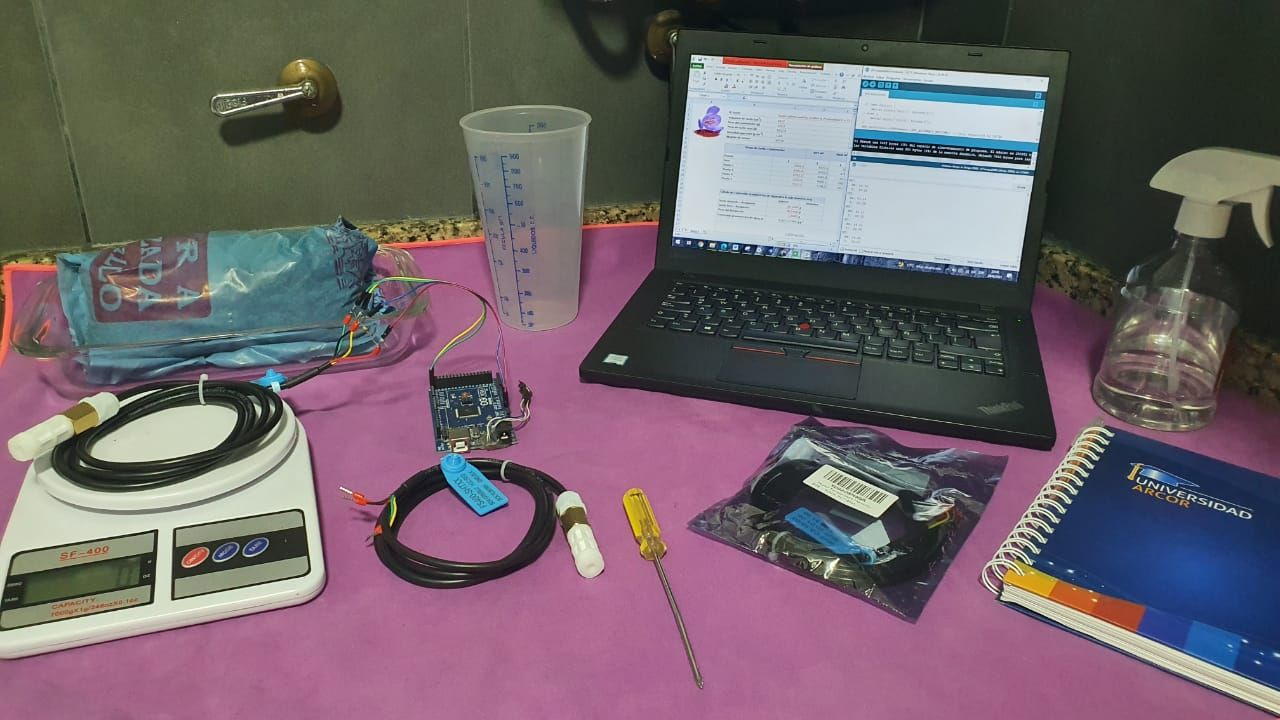
\includegraphics[width=\textwidth]{imagenes/imagenes calibracion/materiales.jpg}
    \caption{Materiales utilizados.}
    \label{fig:materiales}
\end{figure}

\subsection{Procedimiento}

\subsubsection{Preparación de la muestra}

\begin{enumerate}

    \item Pesar el recipiente (limpio y seco) donde se almacenará la muestra.
    \item Debemos obtener la muestra a sensar. Para ello tenemos dos opciones, siendo la primera tomarla directamente del suelo a analizar, empleando un recipiente/sacabocados de volumen conocido; o bien colocando la tierra de propiedades conocidas en un recipiente y compactándola hasta alcanzar la densidad requerida.
    \item Tomar una sub muestra de 10 gramos usando una cuchara o herramienta similar y colocarlo en un recipiente para secado.
    \item Pesar la sub muestra + recipiente (de peso conocido) $M_{wet+recip_B}$ y taparla para evitar la perdida de humedad. Guardarla para su posterior secado.
    \item Anotar el peso ($M_{wet}$) y volumen ($V_{soil}$) de la muestra principal.
    \item Remover objetos grandes que puedan alterar las mediciones, como ser piedras, siempre y cuando no alteren la naturaleza de la muestra.
    \item En caso de ser suelos muy arcillosos o finos, tomar una medición de la altura que ocupa dentro del recipiente, ya que posteriormente su volumen puede cambiar al agregarle agua, por lo que sabiendo la altura se puede llegar a calcular una corrección.
    
\end{enumerate}

\begin{figure}[H]
    \centering
    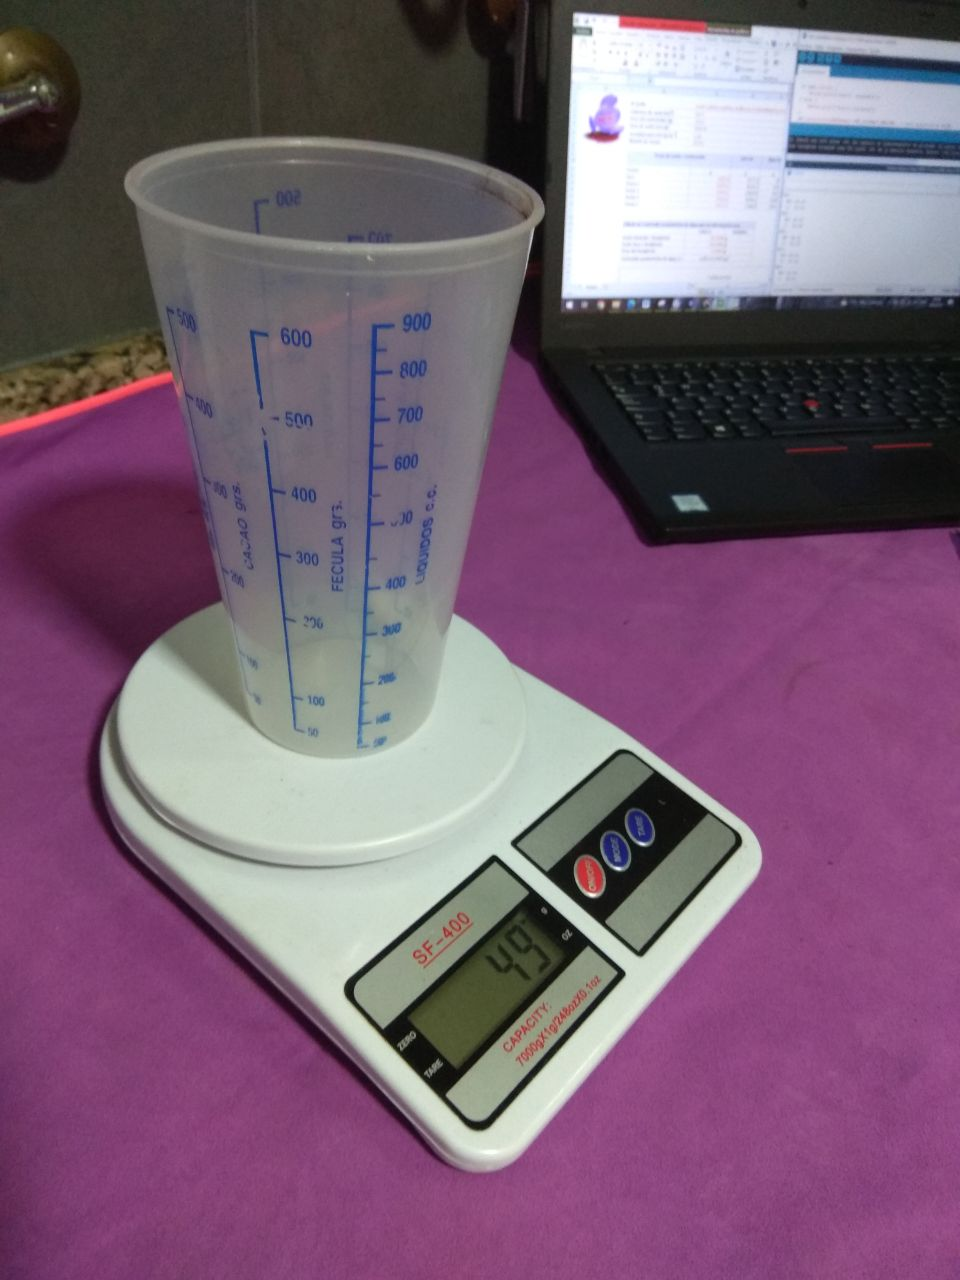
\includegraphics[width=0.5\textwidth]{imagenes/imagenes calibracion/pesovaso.jpg}
    \caption{Pesaje del recipiente.}
    \label{fig:pesaje_vaso}
\end{figure}


\subsubsection{Secado}

\begin{enumerate}

    \item Hornear la muestra principal a 110\degree C hasta lograr que esté completamente seca, variando el tiempo según el peso de muestra. Es recomendable esparcir la tierra en finas capas sobre una bandeja para lograr un secado mas rápido y uniforme.
    \item Sacar del horno y dejar enfriar por 2 horas.
    \item Pesar el suelo seco para obtener $M_{dry}$.
    \item Calcular la densidad aparente del suelo con la ecuación \ref{eqn:bulk_den}.
    
\end{enumerate}

\begin{figure}[h!]
    \centering
    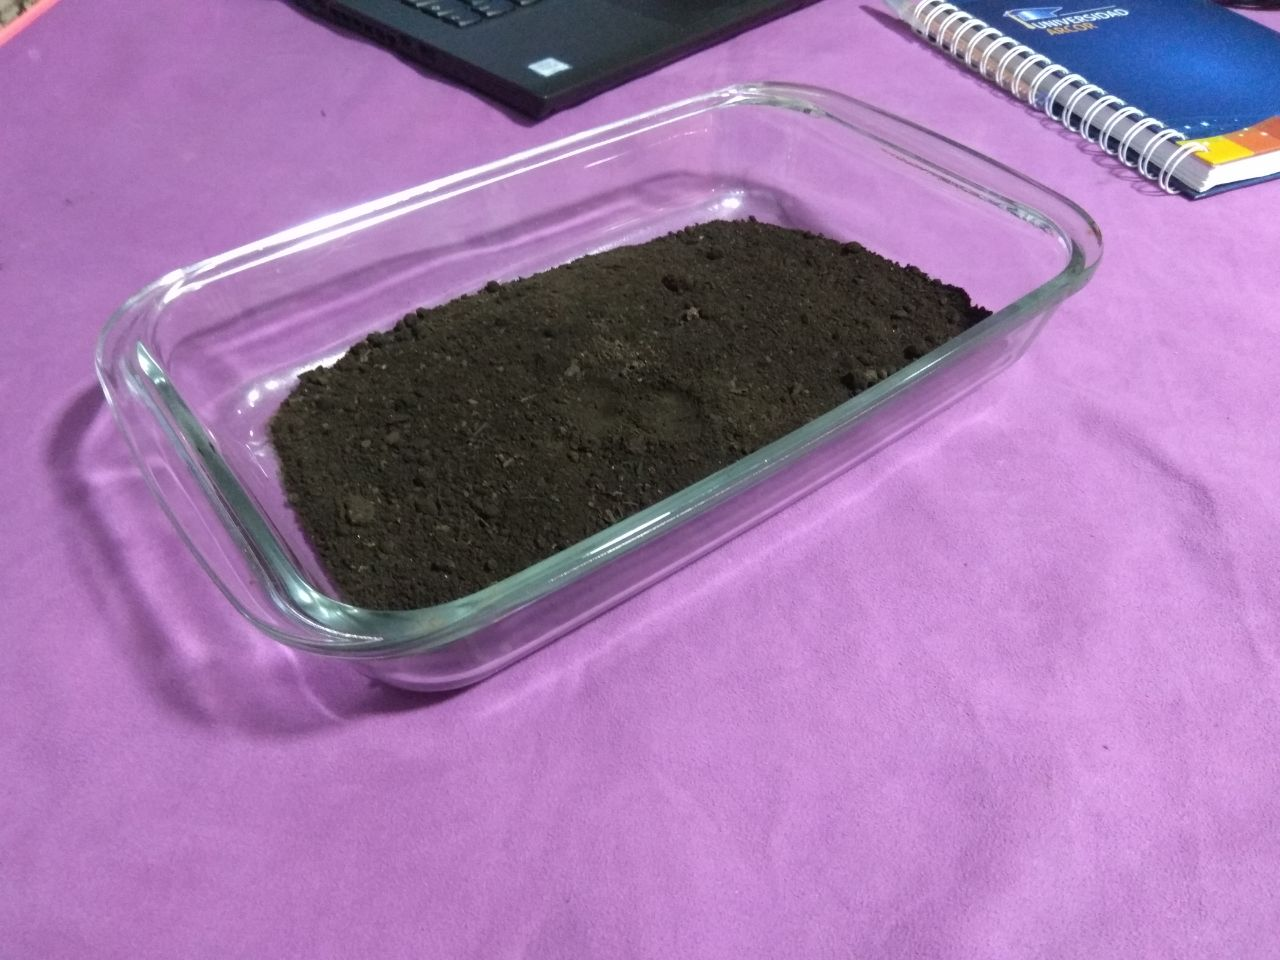
\includegraphics[width=0.5\textwidth]{imagenes/imagenes calibracion/horneado.jpg}
    \caption{Secado de tierra en horno.}
    \label{fig:secado}
\end{figure}
\newpage
\subsubsection{Calibración}

\begin{enumerate}

    \item Colocar la tierra seca en el contenedor para calibración, respetando la densidad y compactación necesaria. Para esto se recomienda ir depositando de a finas capas y compactándolas poco a poco.
    
    \item Introducir el sensor en la muestra, teniendo mucho cuidado de que no queden holguras con aire. Es muy importante que tenga un contacto pleno con la muestra para obtener mediciones acertadas. Se recomienda usar un tutor para hacer el hueco donde tiene que entrar el sensor. Este tiene que quedar completamente dentro de la tierra. Evitar colocarlo en un agujero usado por otro sensor anteriormente.
    \item Conectar el sensor al dispositivo de adquisición y anotar los valores RAW obtenidos.
    \item Retirar el sensor.
    \item Regar la tierra siguiendo una proporción de 1ml de agua por cada 10 ml de tierra, lo que aumentará en un 10\% el contenido de agua volumétrico ($V_{WC}$). Regar lo mas pareja posible la superficie.
    \item Cuidadosamente mezclar la tierra con una cuchara o herramienta similar hasta lograr una consistencia y humedad homogénea.
    \item Repetir los pasos de 2 a 6 hasta lograr la saturación de la tierra, proceso que puede llevar entre 4 y 6 lecturas, con una demora en la adquisición de una hora para cada una.
    \item Es importante destacar que la densidad y compactación de suelo debe mantenerse a lo largo de la prueba, logrando esto asegurándonos de que el volumen de la muestra se mantenga constante sin importar el contenido de agua agregada.
    
\end{enumerate}

\begin{figure}[H]
    \centering
    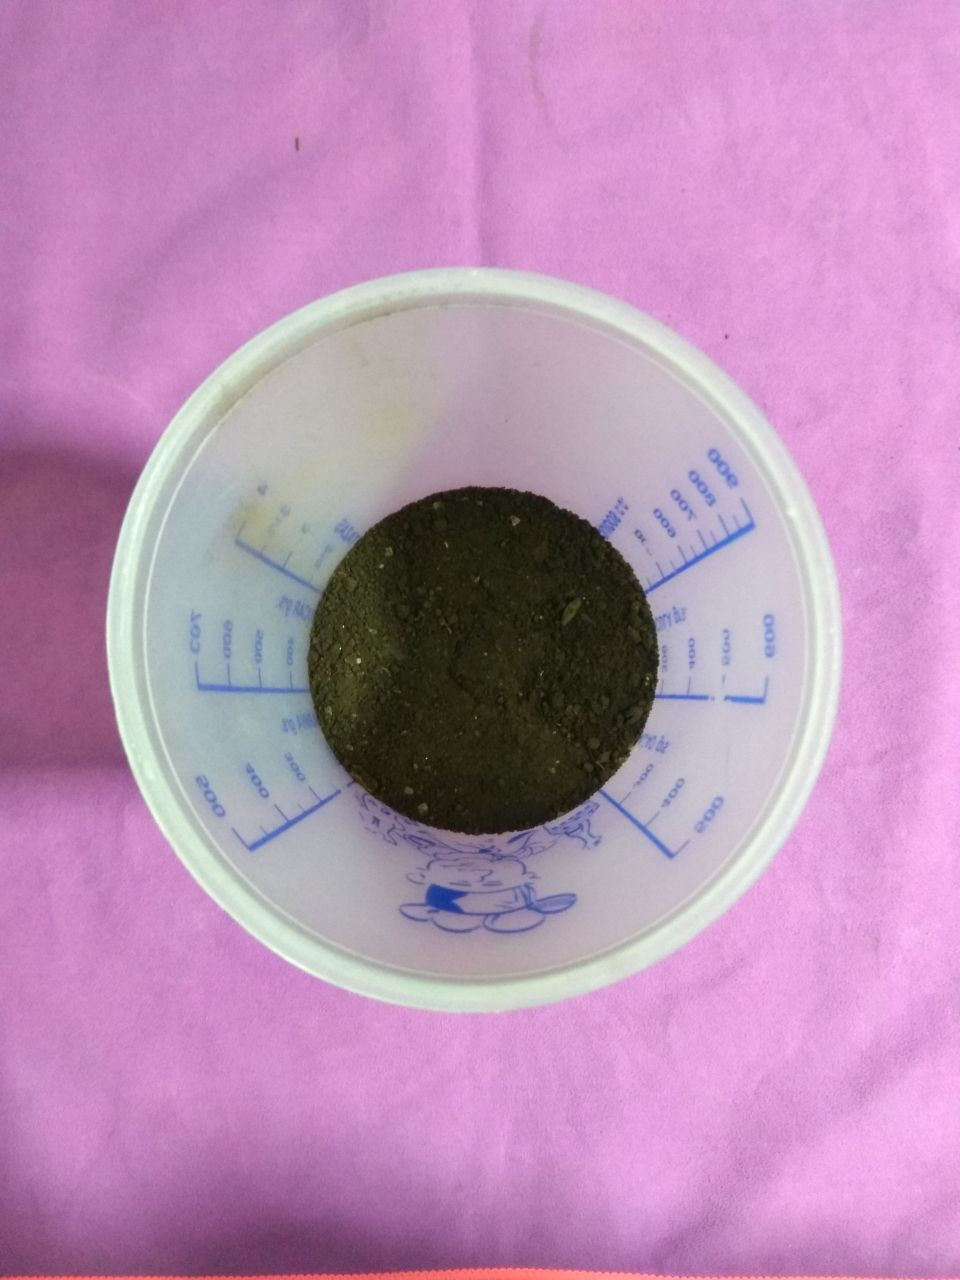
\includegraphics[width=0.45\textwidth]{imagenes/imagenes calibracion/vasolleno.jpg}
    \caption{Recipiente con tierra a medir.}
    \label{fig:vaso_lleno}
\end{figure}

\begin{figure}[H]
    \centering
    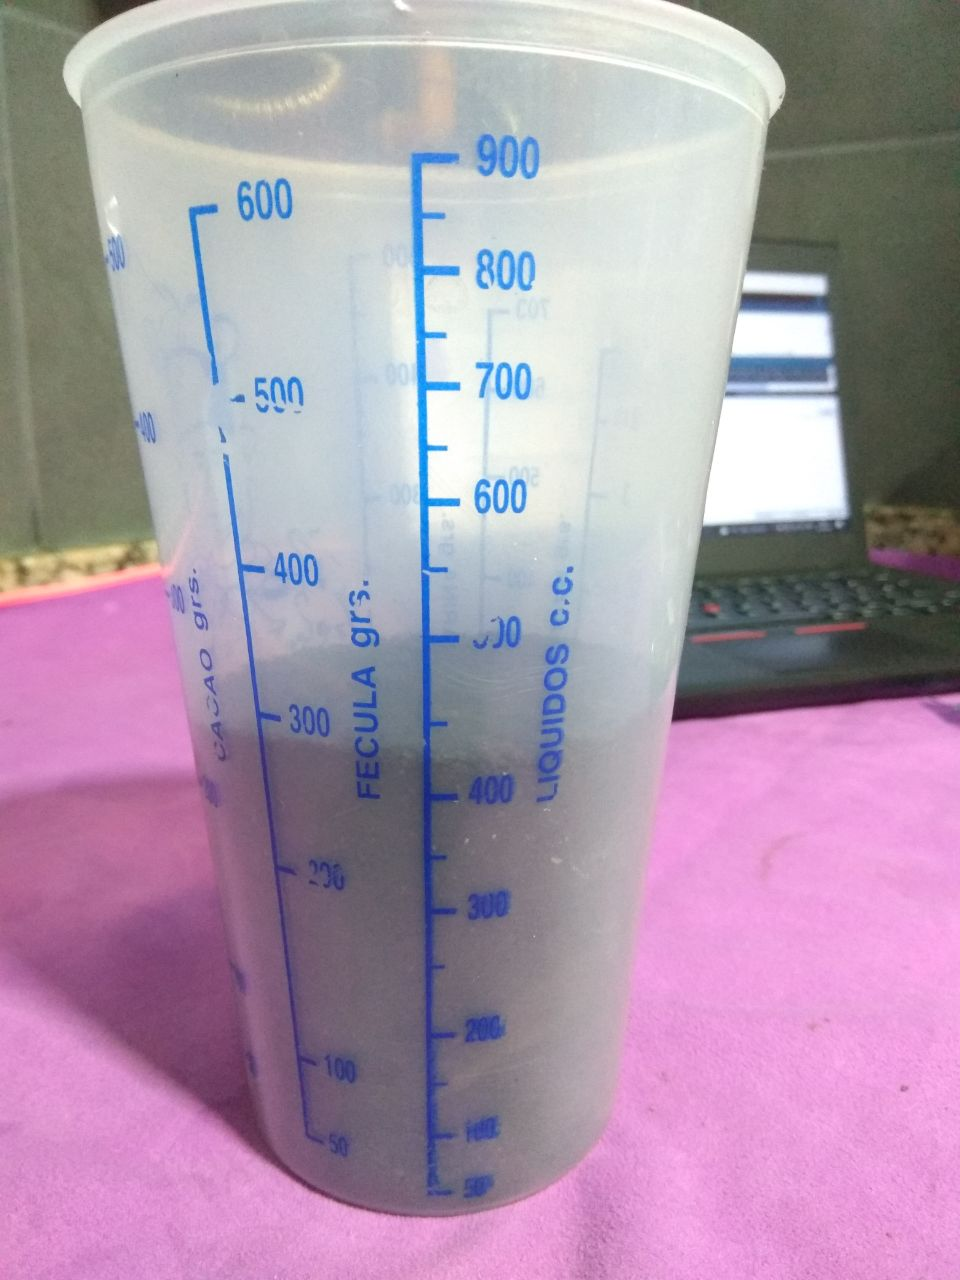
\includegraphics[width=0.45\textwidth]{imagenes/imagenes calibracion/medidavaso.jpg}
    \caption{Volumen de tierra a medir.}
    \label{fig:volumen}
\end{figure}

\begin{figure}[H]
    \centering
    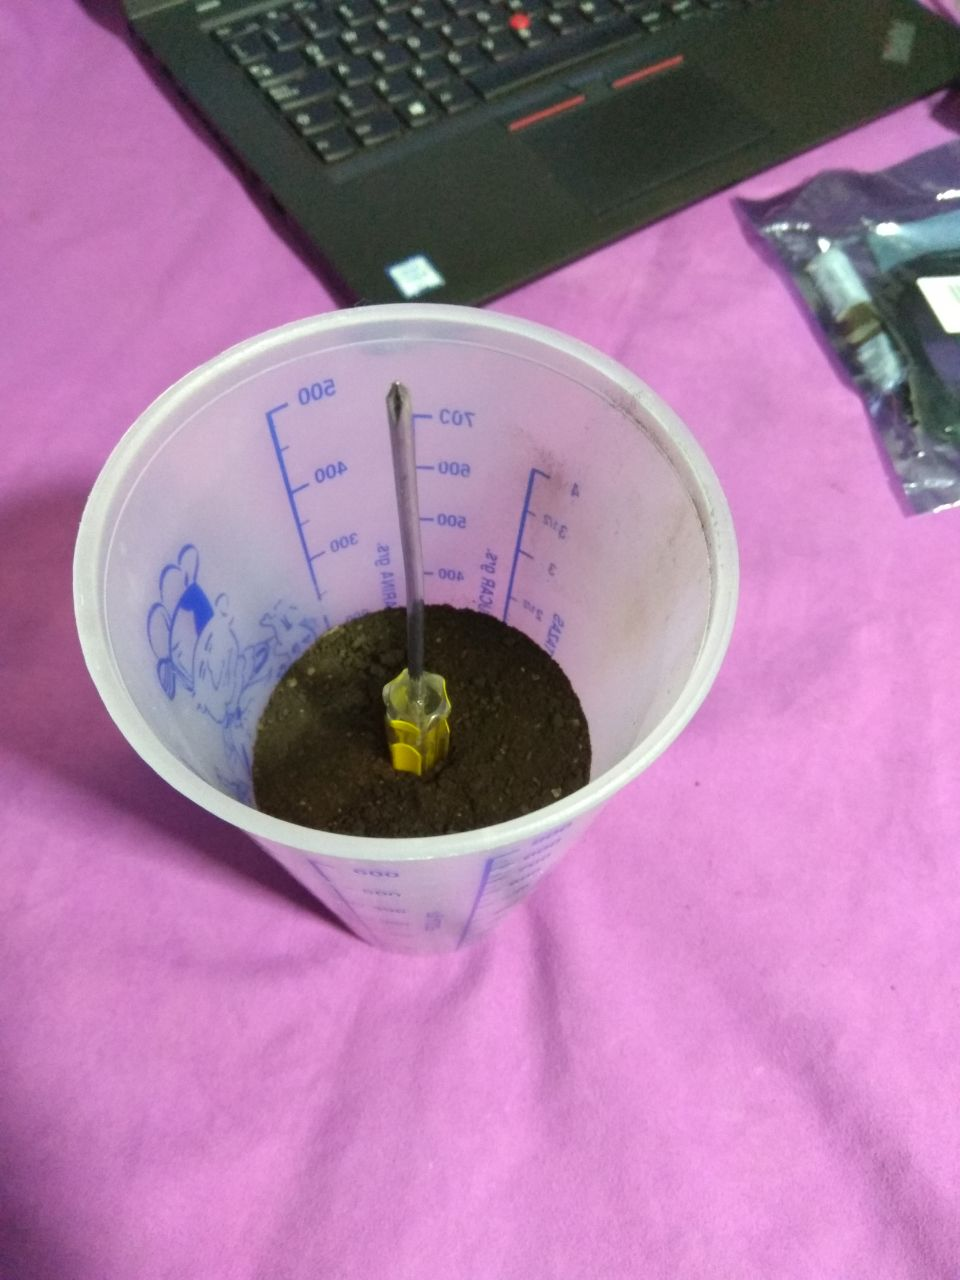
\includegraphics[width=0.45\textwidth]{imagenes/imagenes calibracion/tutor.jpg}
    \caption{Tutor para preparación de suelo.}
    \label{fig:tutor}
\end{figure}

\begin{figure}[H]
    \centering
    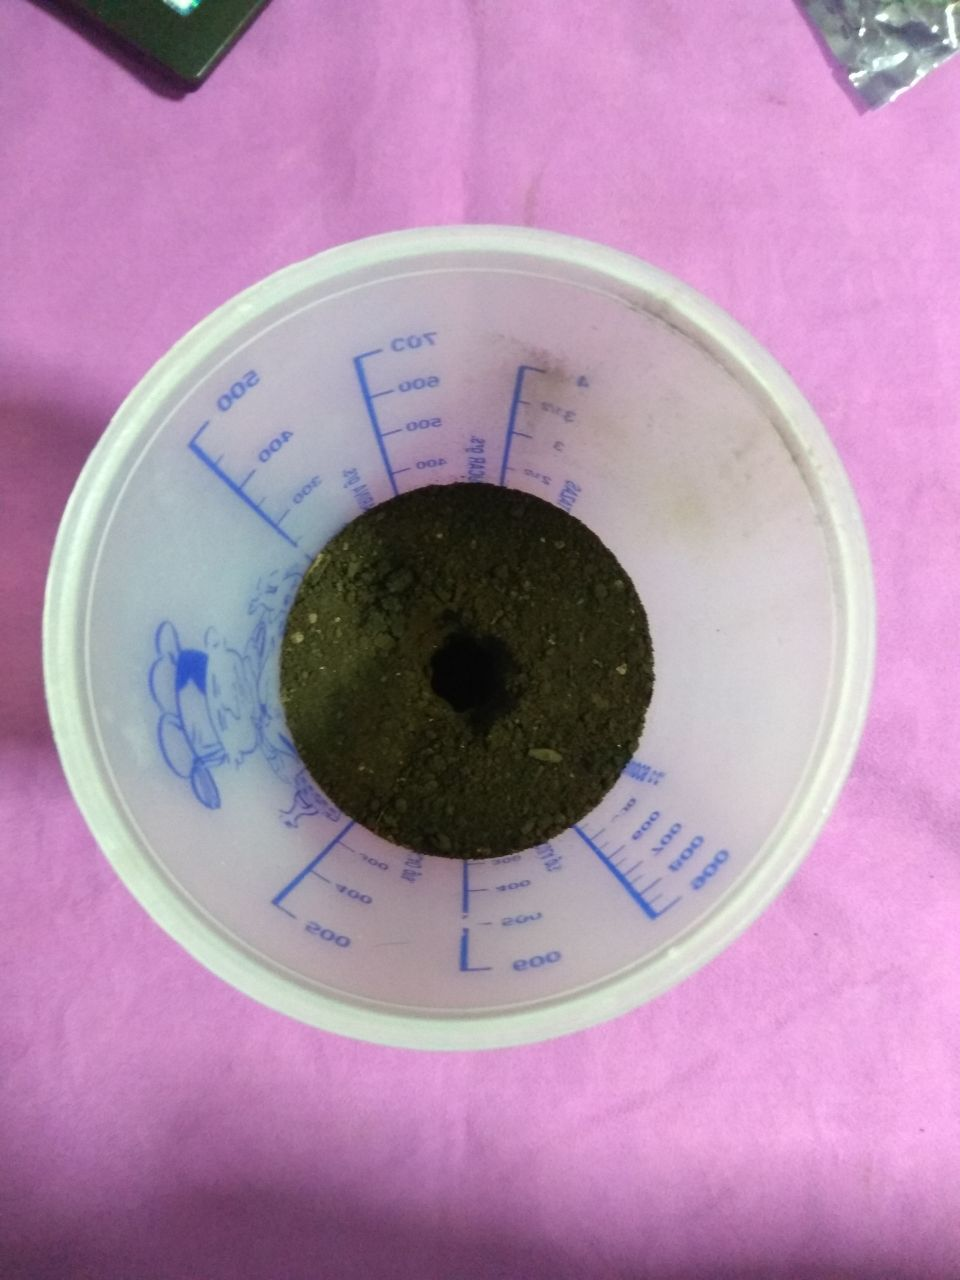
\includegraphics[width=0.45\textwidth]{imagenes/imagenes calibracion/hueco.jpg}
    \caption{Hueco para la inserción del sensor.}
    \label{fig:hueco}
\end{figure}

\begin{figure}[H]
    \centering
    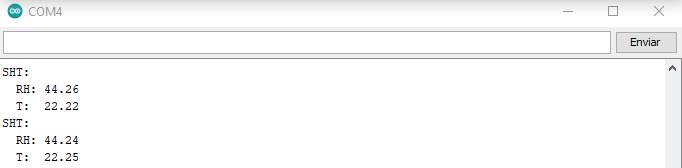
\includegraphics[width=\textwidth]{imagenes/imagenes calibracion/medidas.PNG}
    \caption{Captura de algunas mediciones tomadas.}
    \label{fig:mediciones}
\end{figure}

\subsubsection{Sub-muestra}

\begin{enumerate}

    \item Secar la sub-muestra de 10 gramos obtenida al principio, colocándola en el horno a 105 \degree C por 24 horas, duplicándose ese tiempo si se trata de tierra con alto componente orgánico, siendo necesario en esos casos usar una temperatura de 65 \degree C.
    \item Sacar del horno y dejar enfriar por 2 horas.
    \item Pesar el suelo seco para obtener $M_{dry+recip_B}$.
    

    
\end{enumerate}

\subsubsection{Cálculo y resultados}

\begin{enumerate}

    \item Todas las mediciones obtenidas, sean de peso, volumen o humedad y colocarlas en la tabla de excel para tal fin.
    \item Interpretar el gráfico de la recta de respuesta del sensor y compararlo con el del datasheet para verificar la correlación.
   
\end{enumerate}

\begin{figure}[H]
    \centering
    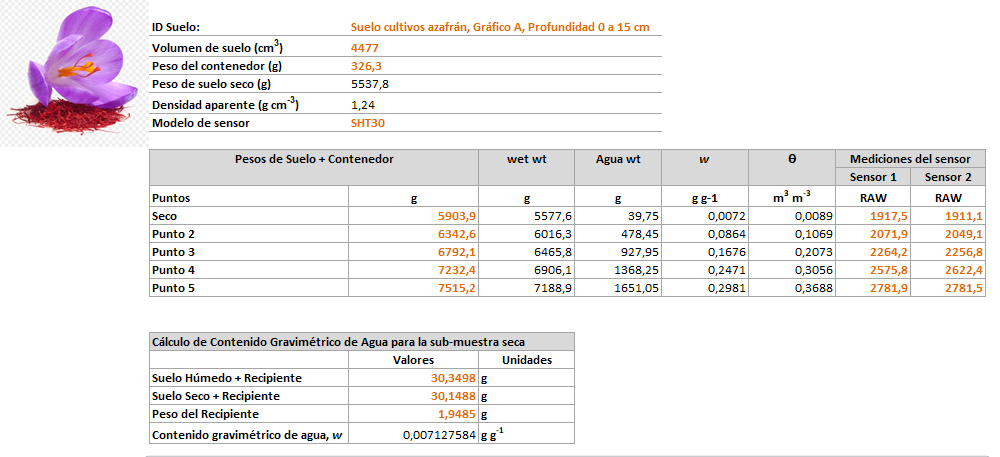
\includegraphics[width=\textwidth]{imagenes/imagenes calibracion/planilla.PNG}
    \caption{Planilla de excel usada para cálculos.}
    \label{fig:planilla}
\end{figure}

\begin{figure}[H]
    \centering
    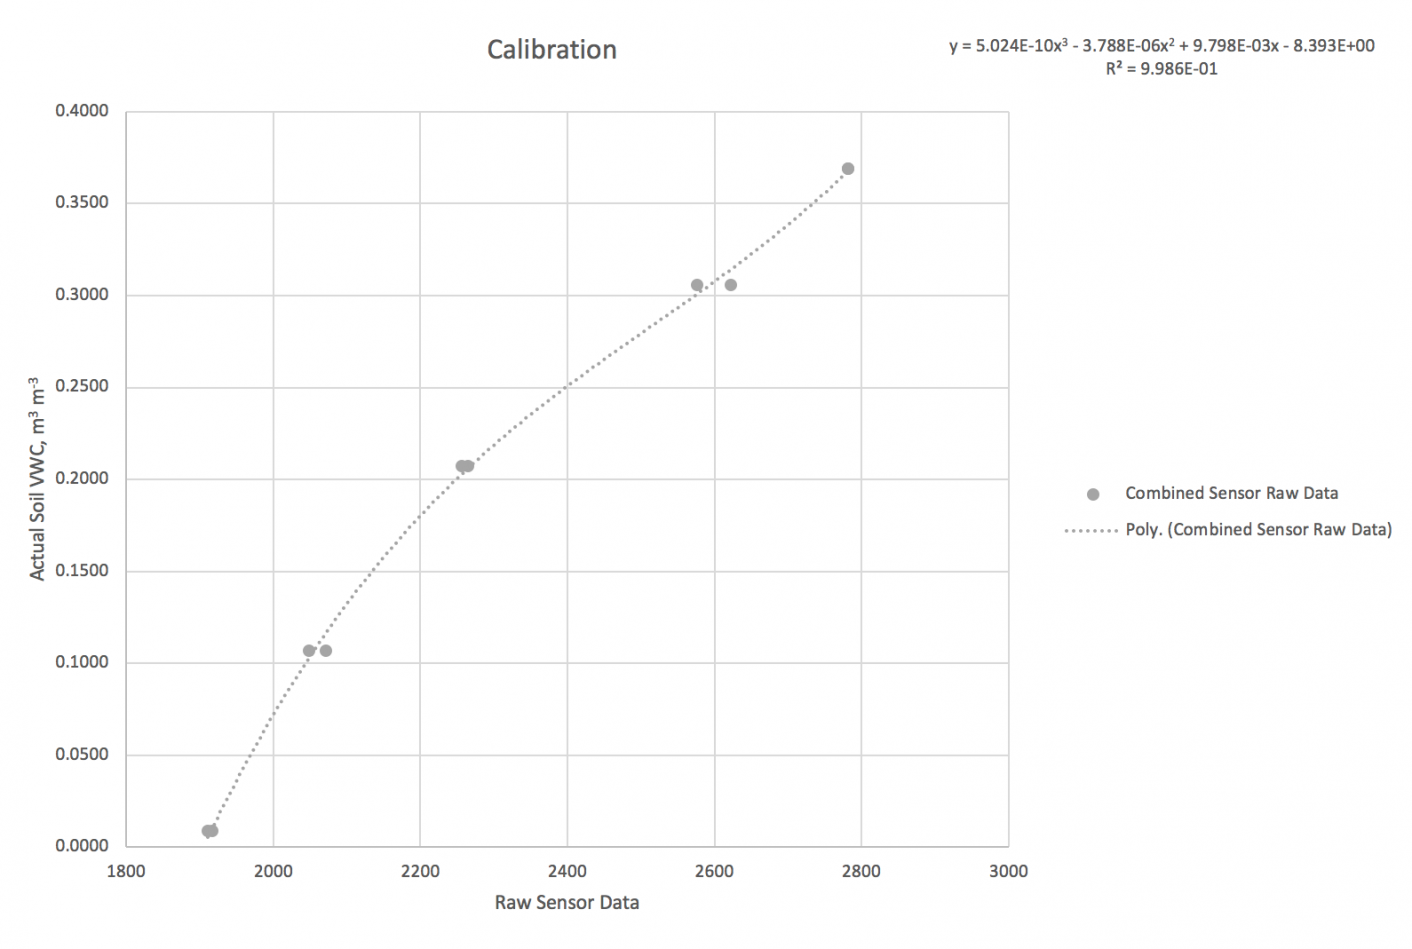
\includegraphics[width=\textwidth]{imagenes/imagenes calibracion/respuesta.png}
    \caption{Curva de respuesta del sensor.}
    \label{fig:respuesta}
\end{figure}



\subsection{Cálculos}

El contenido volumétrico del agua se define como el volumen de agua por volumen de suelo, donde $\theta$ representa el contenido volumétrico de agua, medido en $\frac{cm^3}{cm^3}$.

Otros conceptos que usaremos en este proceso son el volumen de agua, representado con $V_W$ y medido en $cm^3$, y volumen total, que en este caso hace referencia a la capacidad total del contenedor usado para tomar la muestra, representado por $V_T$ y medido en $cm^3$.

\begin{equation}
    \theta = \frac{V_w}{V_t}
    \label{eqn:cont_volum}
\end{equation}

Para calcular el volumen de agua, primero es necesario encontrar la cantidad inicial de agua en nuestra muestra, que se calcula restando el peso total del agua de la muestra, obtenida al multiplicar el peso de la muestra secada por el contenido gravimétrico de agua que se encontró a partir de la sub-muestra de la sección 3.2.4.

\begin{equation}
    m_{soil, sample} = m_{soil, sub-sample} - (m_{soil, sub-sample} \cdot w)
\end{equation}

Donde $m_{soil, sub-sample}$ es la masa de suelo con la que comenzamos y $w$ el contenido gravimétrico de agua calculado a partir de la sub-muestra.

\begin{equation}
    w = \frac{m_{soil, sub-sample}-m_{soil, sample}}{m_{soil, sample}}
\end{equation}

Luego, para encontrar $V_w$ para cada punto de calibración, hay que restar el peso del contenedor y el de $m_{soil, sample}$ del peso total de la muestra.

\begin{equation}
    m_w=m_{total}-m_{soil, sample}
\end{equation}

\begin{equation}
    V_w=\frac{m_w}{\rho_w}
\end{equation}

Dónde $m_w$ es la masa de agua, $m_total$ es la masa de suelo húmedo medida en gramos, $m_{soil, sample}$ es la masa de la muestra secada en horno y $\rho$ es la densidad de agua considerada como $\frac{1gr}{cm^3}$.

Si usamos $V_t$, podemos calcular el contenido volumétrico de agua y la densidad aparente del suelo mediante la ecuación \ref{eqn:cont_volum}, estando esta última definida como la densidad de suelo seco, representada como $\rho_b$ y medida en $\frac{g}{cm^3}$.

\begin{equation}
    \rho_b = \frac{m_{dry}}{V_{soil}}
    \label{eqn:bulk_den}
\end{equation}

Todo lo anterior, en conjunto con la tabla de excel que se encuentra adjunta, permiten realizar la verificación de calibración de nuestro sensor, siendo esto apreciable en el gráfico presente en esta última, el cual usa la herramienta de tendencia para interconectar las mediciones obtenidas y obtener la respuesta de nuestro sensor, la cual puede ser lineal, variando en casos donde la tierra presente un alto contenido de materia orgánica.
